\documentclass{article}
\usepackage{minted}
\usepackage[T1]{fontenc}
\usepackage{polski}
\usepackage[utf8]{inputenc}
\usepackage[polish]{babel}
\usepackage[parfill]{parskip}
\usepackage[a4paper, total={6in, 8in}]{geometry}
\usepackage{graphicx}
\graphicspath{ {./images/} }

\title{System zarządzania partią polityczną - dokumentacja}
\author{Patryk Kumor}


\begin{document}
  \maketitle
  \newpage
  \tableofcontents
  \newpage


\section{Potrzebne pakiety i uruchomienie programu}

\subsection{ Potrzebne pakiety } 

Program został napisany w Pythonie 2.7, z użyciem następujących bibliotek: 
\begin{itemize}
    \item argparse 
    \item json 
    \item sys 
    \item psycopg2 
\end{itemize}
Wszystkie powyższe moduły, oprócz ostatniego - psycopg2 - powinny być dostarczone wraz z podstawową dystrybucją pythona. \newline
Aby zainstalować psycopg2 należy skorzystać z PIP - package managera do\,\,języka python, w tym celu należy wykonać polecenie:
\begin{minted}{shell}
    \$ pip install psycopg2
\end{minted}

\subsection{ Uruchomienie programu }  
Program do zarządzania partią przyjmuje na wejściu obiekty json, które są odczytywane jako ciąg wywołań funkcji API. \newline
Program rozróżnia kilka typów wywołań: 

\paragraph{}  
Aby wywołać program z odczytem linii zawierających obiekty json (jeden obiekt na linię) ze\,\,standar-dowego wejścia w pętli:
\begin{itemize}
\item dla pierwszego wywołania wraz z flagą init:
\begin{minted}{shell}
    \$ python main.py --init
\end{minted}
\item dla kolejnych wowołań:
\begin{minted}{shell}
    \$ python main.py 
\end{minted}
\end{itemize}

\paragraph{}  
Aby wywołać program wraz z odczytem standardowego wejścia zawartego w pliku (każda linia w\,\,pliku jest obiektem json):
\begin{itemize}
\item dla pierwszego wywołania wraz z flagą init:
\begin{minted}{shell}
    \$ python main.py --init < <input_file>
\end{minted}
\item dla kolejnych wowołań:
\begin{minted}{shell}
    \$ python main.py < <input_file>
\end{minted}
\end{itemize}

\paragraph{}  
Aby wywołać program wraz z odczytem zawartości pliku podanego jako argument (każda linia w\,pliku jest obiektem json) należy użyć flagi -\,-f \newline
(program po skończeniu odczytywania zawartości pliku przechodzi w tryb ciągłego czytania ze standardowego wejścia):
\begin{itemize}
\item dla pierwszego wywołania wraz z flagą init:
\begin{minted}{shell}
    \$ python main.py --init --f <input_file>
\end{minted}
\item dla kolejnych wowołań:
\begin{minted}{shell}
    \$ python main.py --f <input_file>
\end{minted}
\end{itemize}

\paragraph{Zakończenie pracy programu \newline}  
Program kończy się automatycznie w przypadku odczytania całej zawartości pliku,
w przypadku ciągłego odczytywania kolejnych linii program zakończy się gdy zostanie użyty skrót \textbf{ctrl+c}.













\newpage
\section{Model fizyczny}
Program przy swoim pierwszym uruchomieniu (wraz z argumentem -\,-init) po pomyślnym połączeniu z bazą danych
tworzy w niej wszystkie potrzebne mu elementy, które są przedstawione na poniższym rysunku. \newline
(Cały schemat użyty podczas tworzenia zawartości bazy danych zawarty jest w pliku \textbf{base.sql})
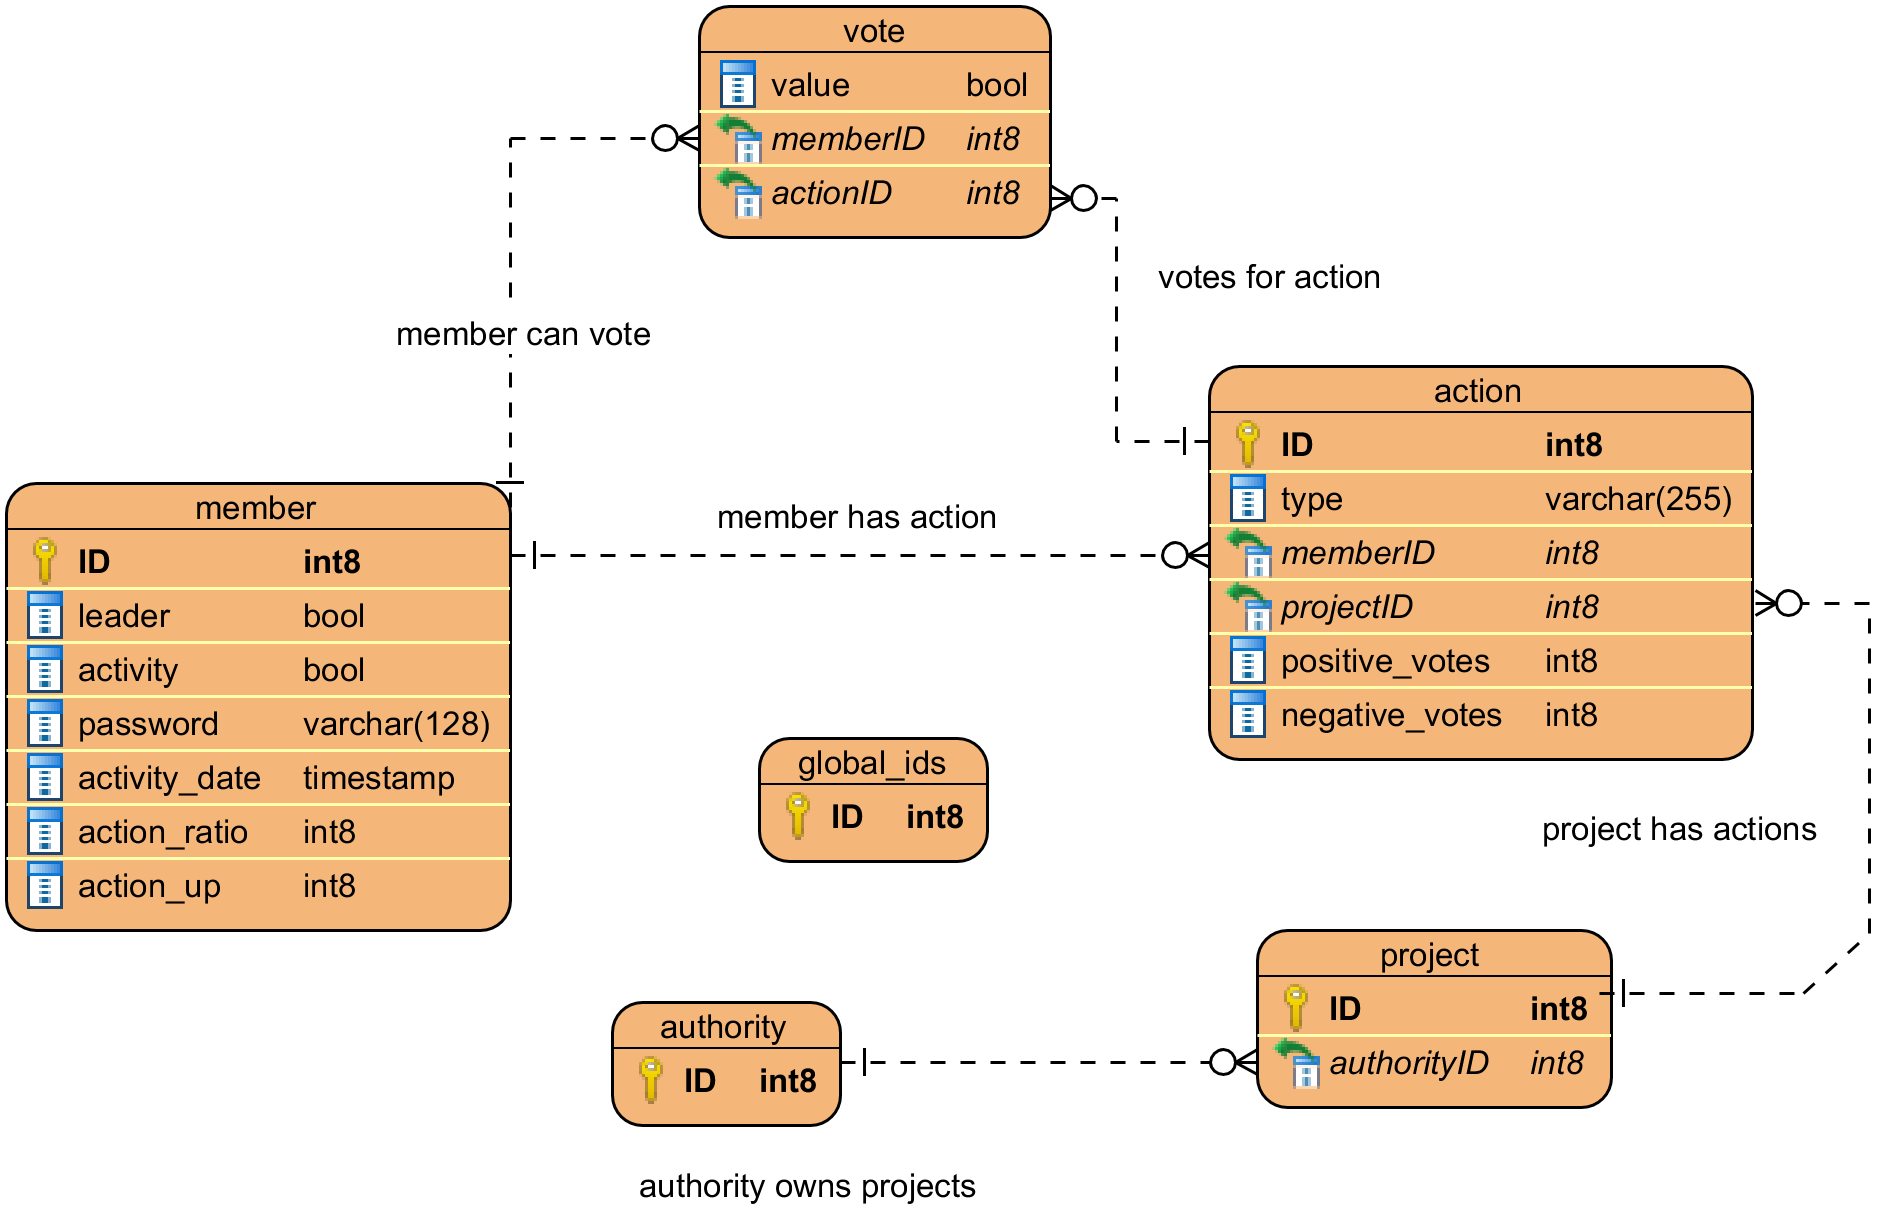
\includegraphics[scale=0.303]{base}  \newline
Użytkownik init, za pomocą którego łączymy się z bazą, posiada wszystkie uprawnienia potrzebne w programie, w tym musi mieć uprawienia do: CREATE TABLE, ADD CONSTRAINT, CREATE user, GRANT <przywilej>.
Użytkownik init również tworzy nową rolę \textbf{app} z uprawieniami UPDATE, INSERT i SELECT na powyższych tabelach. \newline  \newline 
Tabela\textbf{ global\_ids} przechowuje wszystkie id, które zostały użyte do tej pory w programie, dzięki temu jesteśmy w stanie kontrolować globalną unikalność id we wszystkich tabelach \newline
Wytłumaczenie zawartości kolumn, które mogą być niejasne:
\begin{itemize}
\item value w \textbf{vote} - przechowuje informację o tym czy oddany głos jest za (True) czy przeciw (False)
\item positive\_votes i negative\_votes w \textbf{action} - przechowuje informację o oddanej sumarycznej liczbie głosów za/przeciw wobec danej akcji
\item action\_up w \textbf{member} - przechowuje wartość wszystkich głosów upvotes wobec projektów które dany członek utworzył
\item action\_ratio w \textbf{member}- przechowuje wartość (downvotes - upvotes), która potrzebna jest do uznania członka za trolla (jeśli jest dodatnia)
\end{itemize}







\newpage
\section{Implementacja}




\subsection{Dokładny opis wejścia } 
Obiekty json podawane na wejściu mają strukturę: 
\begin{minted}{js}
{     
    <function> : <value>        // nazwa funkcji 
    {
        <arg1> : <value>,        // argumenty funkcji
        <arg2>  : <value>, 
        . . . 
        <argn>  : <value> 
    }
}
\end{minted}
Na przykład funkcja \textbf{open} z argumentami \textbf{<database>} \textbf{<login>} oraz \textbf{<password>} może zostać przekazana na wejściu jako:
\begin{minted}{js}
{ "open": { "database": "student", "login": "app", "password": "qwerty"}}
\end{minted}
Skutkuje to wywołaniem przez program odpowiedniej funkcji przetwarzającej taki obiekt (mającej na celu ustanowienie połączenia z bazą danych wraz z danymi dostępowymi podanymi w argumentach).




\subsection{INIT i kolejne wywołania programu}
Podczas pierwszego uruchomienia programu należy użyć flagi -\,-init.
Podczas uruchomienia -\,-init program pobiera wyłącznie jsony z funkcją open i leader.
Jako pierwszy json pobrany powinien być ten zawierający <open>,\,który definiuje elementy bazy i nawiązuje z nią połączenie,
w przypadku niepowodzenia funkcji obsługującej <open> program zakończy działanie. \newline
Kolejne wywoałania funkcji obsługującej <leader> będą definiować nowe krotki członków, którzy są leaderami. 

Kolejne wywołania programu (bez flagi -\,-init) pobierają i obsługują tylko jsony z funkcjami: 
open, support/protest, upvote/downvote, actions, projects, votes i trolls, 
które zostaną szczegółowo opisane w dalszej części dokumentacji.
Również tutaj w przypadku niepowodzenia <open> program zakończy pracę. 

Program przetwarza wejście parserem json, po czym przekazuje je do funkcji \textbf{if\_case(dic, case)}, 
której argumentem jest nowo utworzony słownik powstały na wskutek działania parsera, oraz nazwa funkcji zawarta w jsonie.

W dalszej części dokumentacji opisane będą sposoby działania funkcji do których zostanie przekierowany program.
Wyjaśnienie oznaczenia we oznaczenia użytego we wszystkich funkcjach głównych odpowiedzialnch za wykonywanie poleceń z jsona:
\begin{itemize}
    \item arg - jest zawartością jsona
    \item conn = psycopg2.connect(args)
    \item cur = conn.cursor()
\end{itemize}







\newpage
\subsection{<open> w funkcjach f\_open\_init i f\_open\_normal}
Pierwsza z funkcji f\_open\_init [przeznaczona jest do wykonania poleceń pierwszego jsona na wejściu] wraz z wykrytą flagą -\,-init, odpowiada za ustanowienie połączenia między bazą danych a\,naszym programem (dzięki rozszerzeniu psycopg2), funkcja ta dodatkowo jest odpowiedzialna za pobranie poleceń bazodanowych z pliku .sql. Funkcja f\_open\_normal jest odpowiadzialna tylko za ustanowienie połączenia z bazą danych.
\paragraph{Opis działania: }
    Na początku należy ustanowić globalne połączenie z bazą danych,
    pobieramy dane logowania z obiektu json. Iniciujemy globalny
    kursor odpowiadający za wykonywanie poleceń bazodanowych. 
    Następnie pobieramy zawartość pliku .sql i wykonujemy execute 
    poleceń towrzących niezbędne elementy bazy danych (wraz z rolą użytkownika app).
    Wykonujemy commit zmian w\,bazie danych, w przypadku wykrycia 
    jakiegokolwiek błędu cofamy wszystkie zmiany i zamykamy program.
\begin{minted}{python}
def f_open_init(arg):
    try:
        global conn
        conn = psycopg2.connect(host="localhost", port="5432",
                                dbname=arg['open']['database'],
                                user=arg['open']['login'],
                                password=arg['open']['password'])
        global cur
        cur = conn.cursor()
        database_create = open('base.sql','r') 
        cur.execute(database_create.read())
        conn.commit()
        print '{"status" : "OK"}'
    except Exception:
        conn.rollback()
        print '{"status" : "ERROR", "debug" : "Polecenie open się nie udało" }' 
        sys.exit(0)  
\end{minted}
Funkcja f\_open\_normal działa na takiej samej zasadzie, ale pomijamy tu pobieranie poleceń z pliku .sql (które powinny być już wcześniej wykonane)






\newpage
\subsection{<leader> w funkcji f\_leader}
Funkcja dodająca leaderów do tabeli member (tylko przy wywołaniach -\,-init)
\paragraph{Opis działania: }
W funkcji pomocniczej \textbf{check\_id} poprzez zapytanie SELECT do bazy danych (wobec tabeli global\_ids) sprawdzamy czy dane nam w argumencie ID jest wolne do użycia.
Jeśli jest wolne to wywołujemy funkcję \textbf{add\_member}, która odpowiada za INSERT krotki do bazy danych o podanych argumentach wejściowych w tabeli member oraz wpisaniu id nowego członka do tabeli global\_ids 
(w\,celi kontroli argumentów kolejnych wywołań - unikalnego id).
\begin{minted}{python}
def f_leader(arg):
    if check_id(arg['leader']['member']): 
        try:
            add_member(arg['leader']['member'],
                       arg['leader']['password'],
                       arg['leader']['timestamp'], 
                       True) # Czy użytkownik jest leaderem
            conn.commit()
            print '{"status" : "OK"}'
        except Exception as err:
            # Rollback jeśli coś poszło nie tak
            conn.rollback()
            print '{"status" : "ERROR", "debug" : "Nie można dodać członka (w funkcji leader)" }' 
    else: 
        print '{"status" : "ERROR",\n "debug" : "ID jest już używany" }'   
\end{minted}

W celu bezpiecznego przechowywania hasła używamy modułu pgcrypto w bazie danych
\begin{minted}{sql}
  crypt(%s, gen_salt('md5'))
\end{minted}







\newpage
\subsection{<protest>/<support> w funkcji f\_protest/f\_support}
Funkcje dodające odpowienio akcję protestacyjne/sprzyjające do projektu (wcześniej zdefiniowanego lub tworząc go podczas działania funkcji)
\paragraph{Opis działania: }
Na starcie w \textbf{authorize\_or\_create\_member} dokonujemy autoryzacji użytkownika
(jeśli istnieje, wpp dodajemy nową krotkę do bazy [wraz z kontrolą poprawności]) sprawdzając jego hasło, potem jego aktywność (przy okazji aktualizując ostatnią aktywność użytkownika za pomocą timestampa [o ile użytkownik nie powinien zostać zamrożony]). \newline
Jeśli podano opcjonalny argument 'authority' jest on pobierany lub wpp oznaczany jako None. Następnie argumenty są przekazywane do funkcji pomocniczej \textbf{create\_action}, która sprawdza wolne ID akcji po czym dodaje je (także z kontrolą poprawności ID, istnienia oraz poprawności projektu/authority etc.) - funkcja powinna zwrócić 1 w przypadku powodzenia wpp 0.\newline
Commit w przypadku powodzenia, rollback w przypadku niepowodzenia, tak jak w poprzedniej funkcji.
\begin{minted}{python}
def f_protest(arg):
    if authorize_or_create_member(arg['protest']['member'],
                                  arg['protest']['password'],
                                  arg['protest']['timestamp']):  
        if 'authority' in arg['protest']: 
            authority = arg['protest']['authority']
        else: 
            authority = None
        if create_action('protest', # analogicznie 'support' w funkcji f_support 
                         arg['protest']['action'],
                         arg['protest']['project'],
                         authority,
                         arg['protest']['member']):
            conn.commit()
            print '{"status" : "OK"}'
        else: 
            conn.rollback()
            print '{"status" : "ERROR", "debug" : "Nie można dodać akcji"}'
    else:
        conn.rollback()
\end{minted}
Funkcja f\_support działa analogicznie wobec f\_protest






\newpage
\subsection{<upvote>/<downvote> w funkcji f\_upvote/f\_downvote }
Funkcje obsługujące system głosowania członków na wcześniej zdefiniowane akcje.
\paragraph{Opis działania: }
Podobnie jak w poprzedniej funkcji dodawania protestu/supportu na starcie sprawdzamy członka, który ma zamiar wykonać działanie (w razie potrzeby dodając krotkę członka do bazy danych). \newline
Następne w funkcji \textbf{vote} dodawana jest krotka do tabeli votes, która pomaga nam rozróżniać członków, którzy już oddali głos na dany projekt, następnie aktualizowane są wartości w tabelach member(autor akcji) i action. W member - aktualizowane wartości ratio autora akcji (w celu późniejszego szukania trolli), w action - suma głosów za/przeciw (w vote sprawdzamy także czy akcja jest uprzednio zdefiniowana). W przypadku gdy wszystko zakończyło się pomyślnie funkcja zwraca 1.
\begin{minted}{python}
def f_upvote(arg):
    if authorize_or_create_member(arg['upvote']['member'],
                                  arg['upvote']['password'], 
                                  arg['upvote']['timestamp']):
        # Oddajemy głos => 1 - upvote, -1 - downvote
        if vote(1, arg['upvote']['member'], arg['upvote']['action']):
            conn.commit()
            print '{"status" : "OK"}'
        else:
            conn.rollback()   
            print '{"status" : "ERROR"}'
    else:
        conn.rollback() 
\end{minted}
f\_downvote - analogicznie.








\newpage
\subsection{<project> w funkcji f\_projects }
Funkcja, którą wywołać może tylko członek z uprawnieniami leadera. Zwraca listę wszystkich akcji wraz z typem, id projektu, id organu władzy oraz z liczbami głosów za i przeciw akcji.
\paragraph{Opis działania: }
Sprawdzamy członka - leadera (w tym jego uprawienia leadera, hasło i aktywność) po czym zgodnie z opcjonalnymi argumentami funkcji votes wysyłamy zapytanie do bazy danych.
Otrzymane krotki formatujemy tak by spełnić wymagania formatu wyjściowego po czym je zwracamy w\,obiekcie json. \newline
\begin{minted}{python}
def f_projects(arg):
    if authorize_leader(arg['projects']['member'], 
                        arg['projects']['password'], 
                        arg['projects']['timestamp']):
        try:
            if 'authority' in arg['projects']:
                cur.execute("""SELECT id, authorityID FROM project 
                               WHERE authorityID = %s ORDER BY id;""",
                           (arg['projects']['authority'],))
            else:
                cur.execute("SELECT id, authorityID FROM project ORDER BY id;")
            wynik =  cur.fetchall()
            print '{"status" : "OK", "data" : %s}' % format_fetch(wynik).replace("'", '"')
        except Exception as err:
            print '{"status" : "ERROR", "debug" : "Błąd podczas zapytania bazodanowego" }' 
    else:
        print '{"status" : "ERROR", "debug" : "Błąd leadera"}'  
\end{minted}







\newpage
\subsection{<votes> w funkcji f\_votes }
Funkcja, którą wywołać może tylko członek z uprawnieniami leadera.
Zwraca listę wszystkich członków (w tym tych, którzy do tej pory nie głosowali) wraz z sumarycznymi liczbami oddanych przez nich głosów za (<upvotes>) i przeciw (downvotes).
\paragraph{Opis działania: }
Sprawdzamy członka - leadera (w tym jego uprawienia leadera, hasło i aktywność) po czym zgodnie z opcjonalnymi argumentami funkcji votes wysyłamy zapytanie do bazy danych.
Otrzymane krotki formatujemy tak by spełnić wymagania formatu wyjściowego po czym je zwracamy w\,obiekcie json. \newline
\begin{minted}{python}
def f_votes(arg):
    if authorize_leader(arg['votes']['member'], 
                        arg['votes']['password'], 
                        arg['votes']['timestamp']):
        try:
            if 'action' in arg['votes']:
                cur.execute("""SELECT mem.id,
                                      sum(case when value then 1 else 0 end) as votes_for,
                                      count(value) as votes 
                                FROM MEMBER as mem LEFT JOIN
                                (SELECT member.id,
                                        vote.value,
                                        action.id as actionid, 
                                        project.id as projectid, 
                                        project.authorityid as authorityid
                                FROM member
                                    LEFT JOIN vote ON(member.id = vote.memberID)
                                    LEFT JOIN action ON(vote.actionid = action.id)
                                    LEFT JOIN project ON(action.projectid = project.id)
                                WHERE action.id = %s
                                ) as foo ON(mem.id = foo.id)
                                GROUP BY mem.id ORDER BY mem.id;""", (arg['votes']['action'],))
            elif 'project' in arg['votes']:
                cur.execute("""SELECT mem.id,
                                      sum(case when value then 1 else 0 end) as votes_for,
                                      count(value) as votes 
                                FROM MEMBER as mem LEFT JOIN
                                (SELECT member.id,
                                        vote.value,
                                        action.id as actionid, 
                                        project.id as projectid, 
                                        project.authorityid as authorityid
                                FROM member
                                    LEFT JOIN vote ON(member.id = vote.memberID)
                                    LEFT JOIN action ON(vote.actionid = action.id)
                                    LEFT JOIN project ON(action.projectid = project.id)
                                WHERE action.projectid = %s
                                ) as foo ON(mem.id = foo.id)
                                GROUP BY mem.id ORDER BY mem.id;""", (arg['votes']['project'],))

            else:
                cur.execute("""SELECT mem.id,
                                      sum(case when value then 1 else 0 end) as votes_for,
                                      count(value) as votes 
                                FROM MEMBER as mem LEFT JOIN
                                (SELECT member.id,
                                        vote.value,
                                        action.id as actionid, 
                                        project.id as projectid, 
                                        project.authorityid as authorityid
                                FROM member
                                    LEFT JOIN vote ON(member.id = vote.memberID)
                                    LEFT JOIN action ON(vote.actionid = action.id)
                                    LEFT JOIN project ON(action.projectid = project.id)
                                ) as foo ON(mem.id = foo.id)
                                GROUP BY mem.id ORDER BY mem.id;""")
            wynik = cur.fetchall()
            wynik = map(helper_votes_tuple, wynik)
            print '{"status" : "OK", "data" : %s}' % format_fetch(wynik).replace("'", '"')  
        except Exception:  
            print '{"status" : "ERROR", "debug" : "Błąd podczas zapytania bazodanowego" }' 
    else:
        print '{"status" : "ERROR", "debug" : "Błąd leadera"}'   
\end{minted}












\newpage
\subsection{<actions> w funkcji f\_actions }
Funkcja, którą wywołać może tylko członek z uprawnieniami leadera. Zwraca listę wszystkich akcji wraz z typem, id projektu, id organu władzy oraz z liczbami głosów za i przeciw akcji.
\paragraph{Opis działania: }
Sprawdzamy członka - leadera (w tym jego uprawienia leadera, hasło i aktywność) po czym zgodnie z opcjonalnymi argumentami funkcji votes wysyłamy zapytanie do bazy danych.
Otrzymane krotki formatujemy tak by spełnić wymagania formatu wyjściowego po czym je zwracamy w\,obiekcie json. \newline
\begin{minted}{python}
def f_actions(arg):
    if authorize_leader(arg['actions']['member'], 
                        arg['actions']['password'], 
                        arg['actions']['timestamp']):
        try:
            if 'type' in arg['actions']:
                if 'project' in arg['actions']:
                    cur.execute("""SELECT action.id, action.type, action.projectID,
                                          project.authorityID, positive_votes,
                                          negative_votes FROM action
                                    JOIN project ON(action.projectID = project.id)
                                    WHERE action.type = %s AND project.id = %s
                                    ORDER BY action.id;""",
                                (arg['actions']['type'],arg['actions']['project']) )
                elif 'authority' in arg['actions']:
                    cur.execute("""SELECT action.id, action.type, action.projectID,
                                          project.authorityID, positive_votes,
                                          negative_votes FROM action
                                    JOIN project ON(action.projectID = project.id)
                                    WHERE action.type = %s AND project.authorityID = %s
                                    ORDER BY action.id;""", 
                                (arg['actions']['type'],arg['actions']['authority']) )
                else:
                    cur.execute("""SELECT action.id, action.type, action.projectID,
                                          project.authorityID, positive_votes,
                                          negative_votes FROM action
                                    JOIN project ON(action.projectID = project.id)
                                    WHERE action.type = %s
                                    ORDER BY action.id;""", (arg['actions']['type'],))
            else:
                if 'project' in arg['actions']:
                    cur.execute("""SELECT action.id, action.type, action.projectID,
                                          project.authorityID, positive_votes,
                                          negative_votes FROM action
                                    JOIN project ON(action.projectID = project.id)
                                    WHERE project.id = %s
                                    ORDER BY action.id;""", (arg['actions']['project'],) )



                elif 'authority' in arg['actions']:
                    cur.execute("""SELECT action.id, action.type, action.projectID,
                                          project.authorityID, positive_votes,
                                          negative_votes FROM action
                                    JOIN project ON(action.projectID = project.id)
                                    WHERE project.authorityID = %s
                                    ORDER BY action.id;""", (arg['actions']['authority'],) )
                else:
                    cur.execute("""SELECT action.id, action.type, action.projectID,
                                          project.authorityID, positive_votes,
                                          negative_votes FROM action
                                    JOIN project ON(action.projectID = project.id)
                                    ORDER BY action.id;""")
            wynik = cur.fetchall()
            print '{"status" : "OK", "data" : %s}' % format_fetch(wynik).replace("'", '"')
        except Exception:
            print '{"status" : "ERROR", "debug" : "Błąd podczas zapytania bazodanowego" }' 
    else:
        print '{"status" : "ERROR", "debug" : "Błąd leadera"}'   
\end{minted}









\newpage
\subsection{<trolls> w funkcji f\_trolls }
Zwraca listę wszystkich użytkowników, którzy zaproponowali akcje mające sumarycznie więcej downvotes niż upvotes wg stanu na chwilę <timestamp>.
\paragraph{Opis działania: }
Na starcie wywołujemy funkcję wykonującą UPDATE aktywność = false w\,przypadku gdy timestamp na wejściu jest oddalony o ponad rok od daty ostatniej aktywności członka. Zwraca 1 gdy nie napotkano na żadne błędy bazy danych. Zadajemy zapytanie do bazy danych, po czym formatujemy krotki wynikowe.
\begin{minted}{python}
def f_trolls(arg):
    if skan(arg['trolls']['timestamp']):                                                  
        cur.execute("""SELECT id, action_up, action_ratio + action_up, activity FROM member
                       WHERE action_ratio > 0 ORDER BY action_ratio desc, id;""")
        wynik = cur.fetchall()
        print '{"status" : "OK", "data" : %s}' % format_fetch(wynik).replace('True', '"true"')
                                                                    .replace('False', '"false"')    
    else:
        print '{"status" : "ERROR", "status" : "błąd bazy danych - update"}' 
\end{minted}





\end{document}
